\documentclass[]{tufte-book}

%  AVI - remove the "double-sided" effect (blank page between chapters) - https://tex.stackexchange.com/questions/111580/removing-an-unwanted-page-between-two-chapters
\let\cleardoublepage\clearpage
%

% ams
\usepackage{amssymb,amsmath}

\usepackage{ifxetex,ifluatex}
\usepackage{fixltx2e} % provides \textsubscript
\ifnum 0\ifxetex 1\fi\ifluatex 1\fi=0 % if pdftex
  \usepackage[T1]{fontenc}
  \usepackage[utf8]{inputenc}
\else % if luatex or xelatex
  \makeatletter
  \@ifpackageloaded{fontspec}{}{\usepackage{fontspec}}
  \makeatother
  \defaultfontfeatures{Ligatures=TeX,Scale=MatchLowercase}
  \makeatletter
  \@ifpackageloaded{soul}{
     \renewcommand\allcapsspacing[1]{{\addfontfeature{LetterSpace=15}#1}}
     \renewcommand\smallcapsspacing[1]{{\addfontfeature{LetterSpace=10}#1}}
   }{}
  \makeatother

\fi

% graphix
\usepackage{graphicx}
\setkeys{Gin}{width=\linewidth,totalheight=\textheight,keepaspectratio}

% booktabs
\usepackage{booktabs}

% url
\usepackage{url}

% hyperref
\usepackage{hyperref}

% units.
\usepackage{units}


\setcounter{secnumdepth}{-1}

% citations
\usepackage{natbib}
\bibliographystyle{plainnat}

% pandoc syntax highlighting
\usepackage{color}
\usepackage{fancyvrb}
\newcommand{\VerbBar}{|}
\newcommand{\VERB}{\Verb[commandchars=\\\{\}]}
\DefineVerbatimEnvironment{Highlighting}{Verbatim}{commandchars=\\\{\}}
% Add ',fontsize=\small' for more characters per line
\newenvironment{Shaded}{}{}
\newcommand{\KeywordTok}[1]{\textcolor[rgb]{0.00,0.44,0.13}{\textbf{#1}}}
\newcommand{\DataTypeTok}[1]{\textcolor[rgb]{0.56,0.13,0.00}{#1}}
\newcommand{\DecValTok}[1]{\textcolor[rgb]{0.25,0.63,0.44}{#1}}
\newcommand{\BaseNTok}[1]{\textcolor[rgb]{0.25,0.63,0.44}{#1}}
\newcommand{\FloatTok}[1]{\textcolor[rgb]{0.25,0.63,0.44}{#1}}
\newcommand{\ConstantTok}[1]{\textcolor[rgb]{0.53,0.00,0.00}{#1}}
\newcommand{\CharTok}[1]{\textcolor[rgb]{0.25,0.44,0.63}{#1}}
\newcommand{\SpecialCharTok}[1]{\textcolor[rgb]{0.25,0.44,0.63}{#1}}
\newcommand{\StringTok}[1]{\textcolor[rgb]{0.25,0.44,0.63}{#1}}
\newcommand{\VerbatimStringTok}[1]{\textcolor[rgb]{0.25,0.44,0.63}{#1}}
\newcommand{\SpecialStringTok}[1]{\textcolor[rgb]{0.73,0.40,0.53}{#1}}
\newcommand{\ImportTok}[1]{#1}
\newcommand{\CommentTok}[1]{\textcolor[rgb]{0.38,0.63,0.69}{\textit{#1}}}
\newcommand{\DocumentationTok}[1]{\textcolor[rgb]{0.73,0.13,0.13}{\textit{#1}}}
\newcommand{\AnnotationTok}[1]{\textcolor[rgb]{0.38,0.63,0.69}{\textbf{\textit{#1}}}}
\newcommand{\CommentVarTok}[1]{\textcolor[rgb]{0.38,0.63,0.69}{\textbf{\textit{#1}}}}
\newcommand{\OtherTok}[1]{\textcolor[rgb]{0.00,0.44,0.13}{#1}}
\newcommand{\FunctionTok}[1]{\textcolor[rgb]{0.02,0.16,0.49}{#1}}
\newcommand{\VariableTok}[1]{\textcolor[rgb]{0.10,0.09,0.49}{#1}}
\newcommand{\ControlFlowTok}[1]{\textcolor[rgb]{0.00,0.44,0.13}{\textbf{#1}}}
\newcommand{\OperatorTok}[1]{\textcolor[rgb]{0.40,0.40,0.40}{#1}}
\newcommand{\BuiltInTok}[1]{#1}
\newcommand{\ExtensionTok}[1]{#1}
\newcommand{\PreprocessorTok}[1]{\textcolor[rgb]{0.74,0.48,0.00}{#1}}
\newcommand{\AttributeTok}[1]{\textcolor[rgb]{0.49,0.56,0.16}{#1}}
\newcommand{\RegionMarkerTok}[1]{#1}
\newcommand{\InformationTok}[1]{\textcolor[rgb]{0.38,0.63,0.69}{\textbf{\textit{#1}}}}
\newcommand{\WarningTok}[1]{\textcolor[rgb]{0.38,0.63,0.69}{\textbf{\textit{#1}}}}
\newcommand{\AlertTok}[1]{\textcolor[rgb]{1.00,0.00,0.00}{\textbf{#1}}}
\newcommand{\ErrorTok}[1]{\textcolor[rgb]{1.00,0.00,0.00}{\textbf{#1}}}
\newcommand{\NormalTok}[1]{#1}

% longtable
\usepackage{longtable,booktabs}

% multiplecol
\usepackage{multicol}

% strikeout
\usepackage[normalem]{ulem}

% morefloats
\usepackage{morefloats}


% tightlist macro required by pandoc >= 1.14
\providecommand{\tightlist}{%
  \setlength{\itemsep}{0pt}\setlength{\parskip}{0pt}}


% title / author / date
\title{Tufte Handout}
\author{JJ Allaire and Yihui Xie}
\date{October 12th, 2017}

\begin{document}

\maketitle




{
\setcounter{tocdepth}{1}
\tableofcontents
}

\chapter{Introduction}\label{introduction}

The Tufte handout style is a style that Edward Tufte uses in his books
and handouts. Tufte's style is known for its extensive use of sidenotes,
tight integration of graphics with text, and well-set typography. This
style has been implemented in LaTeX and HTML/CSS\footnote{See Github
  repositories
  \href{https://github.com/tufte-latex/tufte-latex}{tufte-latex} and
  \href{https://github.com/edwardtufte/tufte-css}{tufte-css}},
respectively. We have ported both implementations into the
\href{https://github.com/rstudio/tufte}{\textbf{tufte} package}. If you
want LaTeX/PDF output, you may use the \texttt{tufte\_handout} format
for handouts, and \texttt{tufte\_book} for books. For HTML output, use
\texttt{tufte\_html}. These formats can be either specified in the YAML
metadata at the beginning of an R Markdown document (see an example
below), or passed to the \texttt{rmarkdown::render()} function. See
\citet{R-rmarkdown} more information about \textbf{rmarkdown}.

\begin{Shaded}
\begin{Highlighting}[]
\OtherTok{---}
\FunctionTok{title:}\AttributeTok{ }\StringTok{"An Example Using the Tufte Style"}
\FunctionTok{author:}\AttributeTok{ }\StringTok{"John Smith"}
\FunctionTok{output:}
  \FunctionTok{tufte:}\AttributeTok{:tufte_handout: default}
  \FunctionTok{tufte:}\AttributeTok{:tufte_html: default}
\OtherTok{---}
\end{Highlighting}
\end{Shaded}

There are two goals of this package:

\begin{enumerate}
\def\labelenumi{\arabic{enumi}.}
\tightlist
\item
  To produce both PDF and HTML output with similar styles from the same
  R Markdown document;
\item
  To provide simple syntax to write elements of the Tufte style such as
  side notes and margin figures, e.g.~when you want a margin figure, all
  you need to do is the chunk option \texttt{fig.margin\ =\ TRUE}, and
  we will take care of the details for you, so you never need to think
  about
  \texttt{\textbackslash{}begin\{marginfigure\}\ \textbackslash{}end\{marginfigure\}}
  or
  \texttt{\textless{}span\ class="marginfigure"\textgreater{}\ \textless{}/span\textgreater{}};
  the LaTeX and HTML code under the hood may be complicated, but you
  never need to learn or write such code.
\end{enumerate}

If you have any feature requests or find bugs in \textbf{tufte}, please
do not hesitate to file them to
\url{https://github.com/rstudio/tufte/issues}. For general questions,
you may ask them on StackOverflow:
\url{http://stackoverflow.com/tags/rmarkdown}.

\chapter{Headings}\label{headings}

This style provides first and second-level headings (that is,
\texttt{\#} and \texttt{\#\#}), demonstrated in the next section. You
may get unexpected output if you try to use \texttt{\#\#\#} and smaller
headings.

\newthought<span class="newthought">In his later books\footnote{\href{http://www.edwardtufte.com/tufte/books_be}{Beautiful
  Evidence}}, Tufte starts each section with a bit of vertical space, a
non-indented paragraph, and sets the first few words of the sentence in
small caps. To accomplish this using this style, call the
\texttt{newthought()} function in \textbf{tufte} in an \emph{inline R
expression} \texttt{\textasciigrave{}r\ \textasciigrave{}} as
demonstrated at the beginning of this paragraph.\footnote{Note you
  should not assume \textbf{tufte} has been attached to your R session.
  You should either \texttt{library(tufte)} in your R Markdown document
  before you call \texttt{newthought()}, or use
  \texttt{tufte::newthought()}.}

\chapter{Figures}\label{figures}

\section{Margin Figures}\label{margin-figures}

Images and graphics play an integral role in Tufte's work. To place
figures in the margin you can use the \textbf{knitr} chunk option
\texttt{fig.margin\ =\ TRUE}. For example:

\begin{Shaded}
\begin{Highlighting}[]
\KeywordTok{library}\NormalTok{(ggplot2)}
\NormalTok{mtcars2 <-}\StringTok{ }\NormalTok{mtcars}
\NormalTok{mtcars2}\OperatorTok{$}\NormalTok{am <-}\StringTok{ }\KeywordTok{factor}\NormalTok{(}
\NormalTok{  mtcars}\OperatorTok{$}\NormalTok{am, }\DataTypeTok{labels =} \KeywordTok{c}\NormalTok{(}\StringTok{'automatic'}\NormalTok{, }\StringTok{'manual'}\NormalTok{)}
\NormalTok{)}
\KeywordTok{ggplot}\NormalTok{(mtcars2, }\KeywordTok{aes}\NormalTok{(hp, mpg, }\DataTypeTok{color =}\NormalTok{ am)) }\OperatorTok{+}
\StringTok{  }\KeywordTok{geom_point}\NormalTok{() }\OperatorTok{+}\StringTok{ }\KeywordTok{geom_smooth}\NormalTok{() }\OperatorTok{+}
\StringTok{  }\KeywordTok{theme}\NormalTok{(}\DataTypeTok{legend.position =} \StringTok{'bottom'}\NormalTok{)}
\end{Highlighting}
\end{Shaded}

\begin{marginfigure}
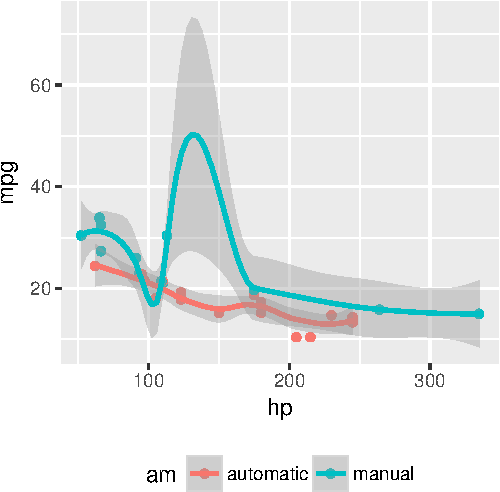
\includegraphics{../reports/APPX_A_Tech_Rpt_2017_files/figure-latex/fig-margin-1} \caption[MPG vs horsepower, colored by transmission]{MPG vs horsepower, colored by transmission.}\label{fig:fig-margin}
\end{marginfigure}

Note the use of the \texttt{fig.cap} chunk option to provide a figure
caption. You can adjust the proportions of figures using the
\texttt{fig.width} and \texttt{fig.height} chunk options. These are
specified in inches, and will be automatically scaled down to fit within
the handout margin.

\section{Arbitrary Margin Content}\label{arbitrary-margin-content}

In fact, you can include anything in the margin using the \textbf{knitr}
engine named \texttt{marginfigure}. Unlike R code chunks
\texttt{\textasciigrave{}\textasciigrave{}\textasciigrave{}\{r\}}, you
write a chunk starting with
\texttt{\textasciigrave{}\textasciigrave{}\textasciigrave{}\{marginfigure\}}
instead, then put the content in the chunk. See an example on the right
about the first fundamental theorem of calculus.

\begin{marginfigure}
We know from \emph{the first fundamental theorem of calculus} that for
\(x\) in \([a, b]\):
\[\frac{d}{dx}\left( \int_{a}^{x} f(u)\,du\right)=f(x).\]
\end{marginfigure}

For the sake of portability between LaTeX and HTML, you should keep the
margin content as simple as possible (syntax-wise) in the
\texttt{marginefigure} blocks. You may use simple Markdown syntax like
\texttt{**bold**} and \texttt{\_italic\_} text, but please refrain from
using footnotes, citations, or block-level elements (e.g.~blockquotes
and lists) there.

Note: if you set \texttt{echo\ =\ FALSE} in your global chunk options,
you will have to add \texttt{echo\ =\ TRUE} to the chunk to display a
margin figure, for example
\texttt{\textasciigrave{}\textasciigrave{}\textasciigrave{}\{marginfigure,\ echo\ =\ TRUE\}}.

\section{Full Width Figures}\label{full-width-figures}

You can arrange for figures to span across the entire page by using the
chunk option \texttt{fig.fullwidth\ =\ TRUE}.

\begin{Shaded}
\begin{Highlighting}[]
\KeywordTok{ggplot}\NormalTok{(diamonds, }\KeywordTok{aes}\NormalTok{(carat, price)) }\OperatorTok{+}\StringTok{ }\KeywordTok{geom_smooth}\NormalTok{() }\OperatorTok{+}
\StringTok{  }\KeywordTok{facet_grid}\NormalTok{(}\OperatorTok{~}\StringTok{ }\NormalTok{cut)}
\end{Highlighting}
\end{Shaded}

\begin{figure*}
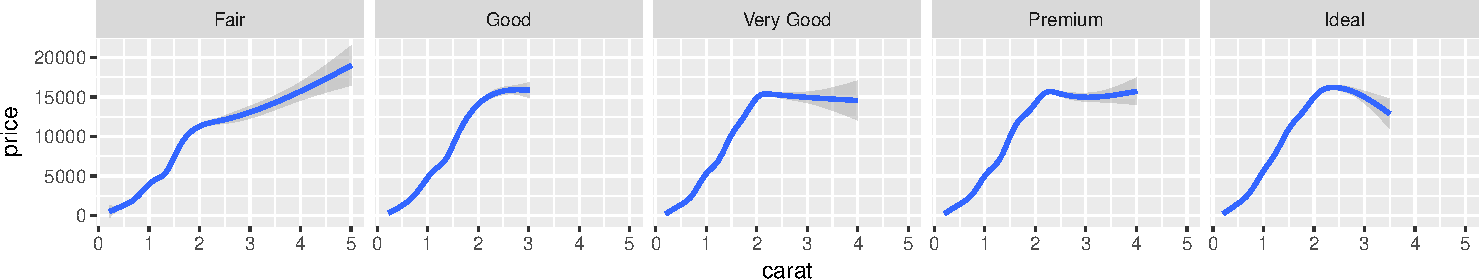
\includegraphics{../reports/APPX_A_Tech_Rpt_2017_files/figure-latex/fig-fullwidth-1} \caption[A full width figure]{A full width figure.}\label{fig:fig-fullwidth}
\end{figure*}

Other chunk options related to figures can still be used, such as
\texttt{fig.width}, \texttt{fig.cap}, \texttt{out.width}, and so on. For
full width figures, usually \texttt{fig.width} is large and
\texttt{fig.height} is small. In the above example, the plot size is
\(10 \times 2\).

\section{Main Column Figures}\label{main-column-figures}

Besides margin and full width figures, you can of course also include
figures constrained to the main column. This is the default type of
figures in the LaTeX/HTML output.

\begin{Shaded}
\begin{Highlighting}[]
\KeywordTok{ggplot}\NormalTok{(diamonds, }\KeywordTok{aes}\NormalTok{(cut, price)) }\OperatorTok{+}\StringTok{ }\KeywordTok{geom_boxplot}\NormalTok{()}
\end{Highlighting}
\end{Shaded}

\begin{figure}
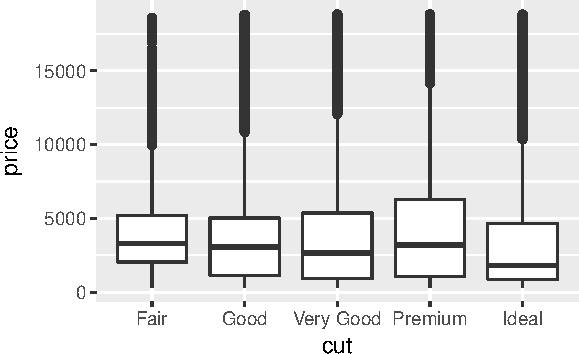
\includegraphics{../reports/APPX_A_Tech_Rpt_2017_files/figure-latex/fig-main-1} \caption[A figure in the main column]{A figure in the main column.}\label{fig:fig-main}
\end{figure}

\chapter{Sidenotes}\label{sidenotes}

One of the most prominent and distinctive features of this style is the
extensive use of sidenotes. There is a wide margin to provide ample room
for sidenotes and small figures. Any use of a footnote will
automatically be converted to a sidenote. \footnote{This is a sidenote
  that was entered using a footnote.}

If you'd like to place ancillary information in the margin without the
sidenote mark (the superscript number), you can use the
\texttt{margin\_note()} function from \textbf{tufte} in an inline R
expression.
\marginnote{This is a margin note.  Notice that there is no number preceding the note.}
This function does not process the text with Pandoc, so Markdown syntax
will not work here. If you need to write anything in Markdown syntax,
please use the \texttt{marginfigure} block described previously.

\chapter{Biblography and References}\label{biblography-and-references}

References can be displayed as margin notes for HTML output. For
example, we can cite R here \citep{R-base}. To enable this feature, you
must set \texttt{link-citations:\ yes} in the YAML metadata, and the
version of \texttt{pandoc-citeproc} should be at least 0.7.2. You can
always install your own version of Pandoc from
\url{http://pandoc.org/installing.html} if the version is not
sufficient. To check the version of \texttt{pandoc-citeproc} in your
system, you may run this in R:

\begin{Shaded}
\begin{Highlighting}[]
\KeywordTok{system2}\NormalTok{(}\StringTok{'pandoc-citeproc'}\NormalTok{, }\StringTok{'--version'}\NormalTok{)}
\end{Highlighting}
\end{Shaded}

If your version of \texttt{pandoc-citeproc} is too low, or you did not
set \texttt{link-citations:\ yes} in YAML, references in the HTML output
will be placed at the end of the output document.

\chapter{Tables}\label{tables}

You can use the \texttt{kable()} function from the \textbf{knitr}
package to format tables that integrate well with the rest of the Tufte
handout style. The table captions are placed in the margin like figures
in the HTML output.

\begin{Shaded}
\begin{Highlighting}[]
\NormalTok{knitr}\OperatorTok{::}\KeywordTok{kable}\NormalTok{(}
\NormalTok{  mtcars[}\DecValTok{1}\OperatorTok{:}\DecValTok{6}\NormalTok{, }\DecValTok{1}\OperatorTok{:}\DecValTok{6}\NormalTok{], }\DataTypeTok{caption =} \StringTok{'A subset of mtcars.'}
\NormalTok{)}
\end{Highlighting}
\end{Shaded}

\begin{longtable}[]{@{}lrrrrrr@{}}
\caption{A subset of mtcars.}\tabularnewline
\toprule
& mpg & cyl & disp & hp & drat & wt\tabularnewline
\midrule
\endfirsthead
\toprule
& mpg & cyl & disp & hp & drat & wt\tabularnewline
\midrule
\endhead
Mazda RX4 & 21.0 & 6 & 160 & 110 & 3.90 & 2.620\tabularnewline
Mazda RX4 Wag & 21.0 & 6 & 160 & 110 & 3.90 & 2.875\tabularnewline
Datsun 710 & 22.8 & 4 & 108 & 93 & 3.85 & 2.320\tabularnewline
Hornet 4 Drive & 21.4 & 6 & 258 & 110 & 3.08 & 3.215\tabularnewline
Hornet Sportabout & 18.7 & 8 & 360 & 175 & 3.15 & 3.440\tabularnewline
Valiant & 18.1 & 6 & 225 & 105 & 2.76 & 3.460\tabularnewline
\bottomrule
\end{longtable}

\chapter{Block Quotes}\label{block-quotes}

We know from the Markdown syntax that paragraphs that start with
\texttt{\textgreater{}} are converted to block quotes. If you want to
add a right-aligned footer for the quote, you may use the function
\texttt{quote\_footer()} from \textbf{tufte} in an inline R expression.
Here is an example:

\begin{quote}
``If it weren't for my lawyer, I'd still be in prison. It went a lot
faster with two people digging.''

\hfill --- Joe Martin
\end{quote}

Without using \texttt{quote\_footer()}, it looks like this (the second
line is just a normal paragraph):

\begin{quote}
``Great people talk about ideas, average people talk about things, and
small people talk about wine.''

--- Fran Lebowitz
\end{quote}

\chapter{Responsiveness}\label{responsiveness}

The HTML page is responsive in the sense that when the page width is
smaller than 760px, sidenotes and margin notes will be hidden by
default. For sidenotes, you can click their numbers (the superscripts)
to toggle their visibility. For margin notes, you may click the circled
plus signs to toggle visibility.

\chapter{More Examples}\label{more-examples}

The rest of this document consists of a few test cases to make sure
everything still works well in slightly more complicated scenarios.
First we generate two plots in one figure environment with the chunk
option \texttt{fig.show\ =\ \textquotesingle{}hold\textquotesingle{}}:

\begin{Shaded}
\begin{Highlighting}[]
\NormalTok{p <-}\StringTok{ }\KeywordTok{ggplot}\NormalTok{(mtcars2, }\KeywordTok{aes}\NormalTok{(hp, mpg, }\DataTypeTok{color =}\NormalTok{ am)) }\OperatorTok{+}
\StringTok{  }\KeywordTok{geom_point}\NormalTok{()}
\NormalTok{p}
\NormalTok{p }\OperatorTok{+}\StringTok{ }\KeywordTok{geom_smooth}\NormalTok{()}
\end{Highlighting}
\end{Shaded}

\begin{figure}
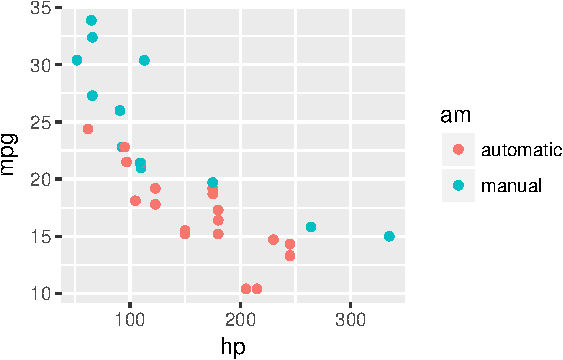
\includegraphics{../reports/APPX_A_Tech_Rpt_2017_files/figure-latex/fig-two-together-1} 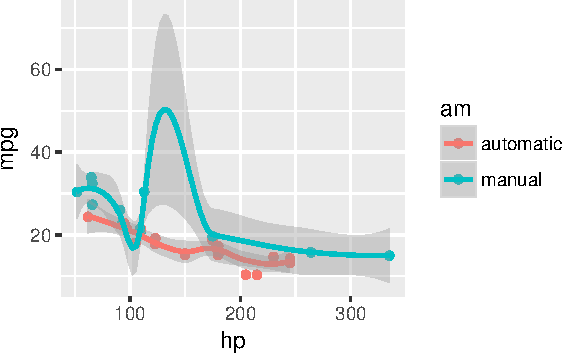
\includegraphics{../reports/APPX_A_Tech_Rpt_2017_files/figure-latex/fig-two-together-2} \caption[Two plots in one figure environment]{Two plots in one figure environment.}\label{fig:fig-two-together}
\end{figure}

Then two plots in separate figure environments (the code is identical to
the previous code chunk, but the chunk option is the default
\texttt{fig.show\ =\ \textquotesingle{}asis\textquotesingle{}} now):

\begin{Shaded}
\begin{Highlighting}[]
\NormalTok{p <-}\StringTok{ }\KeywordTok{ggplot}\NormalTok{(mtcars2, }\KeywordTok{aes}\NormalTok{(hp, mpg, }\DataTypeTok{color =}\NormalTok{ am)) }\OperatorTok{+}
\StringTok{  }\KeywordTok{geom_point}\NormalTok{()}
\NormalTok{p}
\end{Highlighting}
\end{Shaded}

\begin{figure}
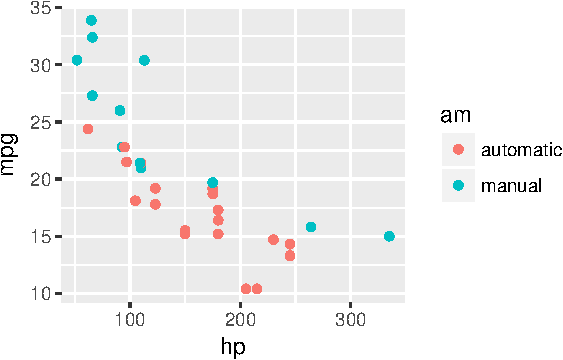
\includegraphics{../reports/APPX_A_Tech_Rpt_2017_files/figure-latex/fig-two-separate-1} \caption[Two plots in separate figure environments (the first plot)]{Two plots in separate figure environments (the first plot).}\label{fig:fig-two-separate1}
\end{figure}

\begin{Shaded}
\begin{Highlighting}[]
\NormalTok{p }\OperatorTok{+}\StringTok{ }\KeywordTok{geom_smooth}\NormalTok{()}
\end{Highlighting}
\end{Shaded}

\begin{figure}
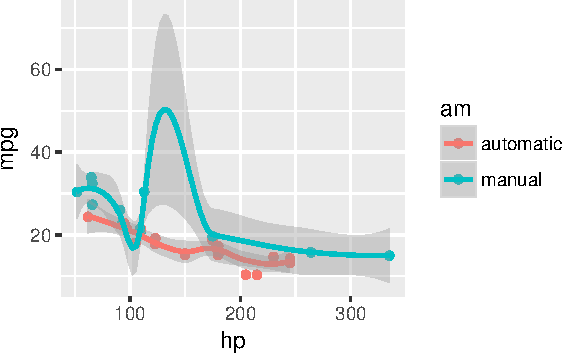
\includegraphics{../reports/APPX_A_Tech_Rpt_2017_files/figure-latex/fig-two-separate-2} \caption[Two plots in separate figure environments (the second plot)]{Two plots in separate figure environments (the second plot).}\label{fig:fig-two-separate2}
\end{figure}

You may have noticed that the two figures have different captions, and
that is because we used a character vector of length 2 for the chunk
option \texttt{fig.cap} (something like
\texttt{fig.cap\ =\ c(\textquotesingle{}first\ plot\textquotesingle{},\ \textquotesingle{}second\ plot\textquotesingle{})}).

Next we show multiple plots in margin figures. Similarly, two plots in
the same figure environment in the margin:

\begin{Shaded}
\begin{Highlighting}[]
\NormalTok{p}
\NormalTok{p }\OperatorTok{+}\StringTok{ }\KeywordTok{geom_smooth}\NormalTok{(}\DataTypeTok{method =} \StringTok{'lm'}\NormalTok{)}
\end{Highlighting}
\end{Shaded}

\begin{marginfigure}
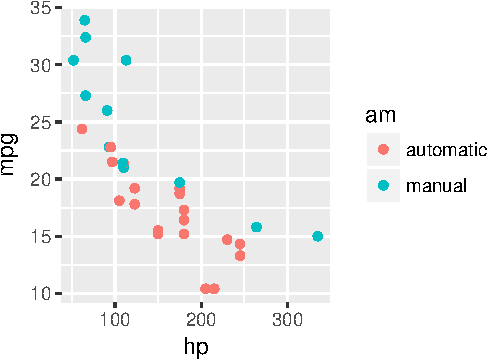
\includegraphics{../reports/APPX_A_Tech_Rpt_2017_files/figure-latex/fig-margin-together-1} 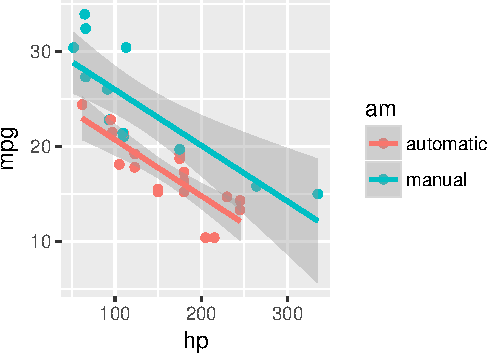
\includegraphics{../reports/APPX_A_Tech_Rpt_2017_files/figure-latex/fig-margin-together-2} \caption[Two plots in one figure environment in the margin]{Two plots in one figure environment in the margin.}\label{fig:fig-margin-together}
\end{marginfigure}

Then two plots from the same code chunk placed in different figure
environments:

\begin{Shaded}
\begin{Highlighting}[]
\NormalTok{knitr}\OperatorTok{::}\KeywordTok{kable}\NormalTok{(}\KeywordTok{head}\NormalTok{(iris, }\DecValTok{15}\NormalTok{))}
\end{Highlighting}
\end{Shaded}

\begin{longtable}[]{@{}rrrrl@{}}
\toprule
Sepal.Length & Sepal.Width & Petal.Length & Petal.Width &
Species\tabularnewline
\midrule
\endhead
5.1 & 3.5 & 1.4 & 0.2 & setosa\tabularnewline
4.9 & 3.0 & 1.4 & 0.2 & setosa\tabularnewline
4.7 & 3.2 & 1.3 & 0.2 & setosa\tabularnewline
4.6 & 3.1 & 1.5 & 0.2 & setosa\tabularnewline
5.0 & 3.6 & 1.4 & 0.2 & setosa\tabularnewline
5.4 & 3.9 & 1.7 & 0.4 & setosa\tabularnewline
4.6 & 3.4 & 1.4 & 0.3 & setosa\tabularnewline
5.0 & 3.4 & 1.5 & 0.2 & setosa\tabularnewline
4.4 & 2.9 & 1.4 & 0.2 & setosa\tabularnewline
4.9 & 3.1 & 1.5 & 0.1 & setosa\tabularnewline
5.4 & 3.7 & 1.5 & 0.2 & setosa\tabularnewline
4.8 & 3.4 & 1.6 & 0.2 & setosa\tabularnewline
4.8 & 3.0 & 1.4 & 0.1 & setosa\tabularnewline
4.3 & 3.0 & 1.1 & 0.1 & setosa\tabularnewline
5.8 & 4.0 & 1.2 & 0.2 & setosa\tabularnewline
\bottomrule
\end{longtable}

\begin{Shaded}
\begin{Highlighting}[]
\NormalTok{p}
\end{Highlighting}
\end{Shaded}

\begin{marginfigure}
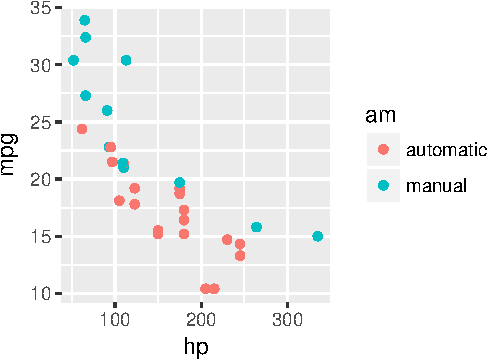
\includegraphics{../reports/APPX_A_Tech_Rpt_2017_files/figure-latex/fig-margin-separate-1} \caption[Two plots in separate figure environments in the margin (the first plot)]{Two plots in separate figure environments in the margin (the first plot).}\label{fig:fig-margin-separate1}
\end{marginfigure}

\begin{Shaded}
\begin{Highlighting}[]
\NormalTok{knitr}\OperatorTok{::}\KeywordTok{kable}\NormalTok{(}\KeywordTok{head}\NormalTok{(iris, }\DecValTok{12}\NormalTok{))}
\end{Highlighting}
\end{Shaded}

\begin{longtable}[]{@{}rrrrl@{}}
\toprule
Sepal.Length & Sepal.Width & Petal.Length & Petal.Width &
Species\tabularnewline
\midrule
\endhead
5.1 & 3.5 & 1.4 & 0.2 & setosa\tabularnewline
4.9 & 3.0 & 1.4 & 0.2 & setosa\tabularnewline
4.7 & 3.2 & 1.3 & 0.2 & setosa\tabularnewline
4.6 & 3.1 & 1.5 & 0.2 & setosa\tabularnewline
5.0 & 3.6 & 1.4 & 0.2 & setosa\tabularnewline
5.4 & 3.9 & 1.7 & 0.4 & setosa\tabularnewline
4.6 & 3.4 & 1.4 & 0.3 & setosa\tabularnewline
5.0 & 3.4 & 1.5 & 0.2 & setosa\tabularnewline
4.4 & 2.9 & 1.4 & 0.2 & setosa\tabularnewline
4.9 & 3.1 & 1.5 & 0.1 & setosa\tabularnewline
5.4 & 3.7 & 1.5 & 0.2 & setosa\tabularnewline
4.8 & 3.4 & 1.6 & 0.2 & setosa\tabularnewline
\bottomrule
\end{longtable}

\begin{Shaded}
\begin{Highlighting}[]
\NormalTok{p }\OperatorTok{+}\StringTok{ }\KeywordTok{geom_smooth}\NormalTok{(}\DataTypeTok{method =} \StringTok{'lm'}\NormalTok{)}
\end{Highlighting}
\end{Shaded}

\begin{marginfigure}
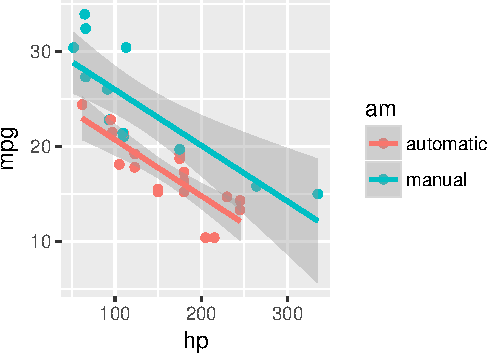
\includegraphics{../reports/APPX_A_Tech_Rpt_2017_files/figure-latex/fig-margin-separate-2} \caption[Two plots in separate figure environments in the margin (the second plot)]{Two plots in separate figure environments in the margin (the second plot).}\label{fig:fig-margin-separate2}
\end{marginfigure}

\begin{Shaded}
\begin{Highlighting}[]
\NormalTok{knitr}\OperatorTok{::}\KeywordTok{kable}\NormalTok{(}\KeywordTok{head}\NormalTok{(iris, }\DecValTok{5}\NormalTok{))}
\end{Highlighting}
\end{Shaded}

\begin{longtable}[]{@{}rrrrl@{}}
\toprule
Sepal.Length & Sepal.Width & Petal.Length & Petal.Width &
Species\tabularnewline
\midrule
\endhead
5.1 & 3.5 & 1.4 & 0.2 & setosa\tabularnewline
4.9 & 3.0 & 1.4 & 0.2 & setosa\tabularnewline
4.7 & 3.2 & 1.3 & 0.2 & setosa\tabularnewline
4.6 & 3.1 & 1.5 & 0.2 & setosa\tabularnewline
5.0 & 3.6 & 1.4 & 0.2 & setosa\tabularnewline
\bottomrule
\end{longtable}

We blended some tables in the above code chunk only as
\emph{placeholders} to make sure there is enough vertical space among
the margin figures, otherwise they will be stacked tightly together. For
a practical document, you should not insert too many margin figures
consecutively and make the margin crowded.

You do not have to assign captions to figures. We show three figures
with no captions below in the margin, in the main column, and in full
width, respectively.

\begin{Shaded}
\begin{Highlighting}[]
\CommentTok{# a boxplot of weight vs transmission; this figure}
\CommentTok{# will be placed in the margin}
\KeywordTok{ggplot}\NormalTok{(mtcars2, }\KeywordTok{aes}\NormalTok{(am, wt)) }\OperatorTok{+}\StringTok{ }\KeywordTok{geom_boxplot}\NormalTok{() }\OperatorTok{+}
\StringTok{  }\KeywordTok{coord_flip}\NormalTok{()}
\end{Highlighting}
\end{Shaded}

\begin{marginfigure}
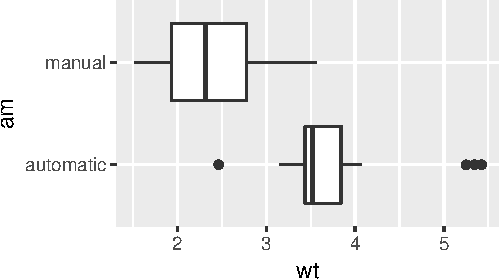
\includegraphics{../reports/APPX_A_Tech_Rpt_2017_files/figure-latex/fig-nocap-margin-1} \end{marginfigure}

\begin{Shaded}
\begin{Highlighting}[]
\CommentTok{# a figure in the main column}
\NormalTok{p <-}\StringTok{ }\KeywordTok{ggplot}\NormalTok{(mtcars, }\KeywordTok{aes}\NormalTok{(wt, hp)) }\OperatorTok{+}\StringTok{ }\KeywordTok{geom_point}\NormalTok{()}
\NormalTok{p}
\end{Highlighting}
\end{Shaded}

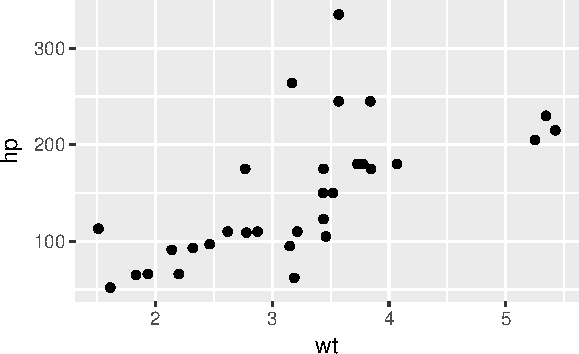
\includegraphics{../reports/APPX_A_Tech_Rpt_2017_files/figure-latex/fig-nocap-main-1}

\begin{Shaded}
\begin{Highlighting}[]
\CommentTok{# a fullwidth figure}
\NormalTok{p }\OperatorTok{+}\StringTok{ }\KeywordTok{geom_smooth}\NormalTok{(}\DataTypeTok{method =} \StringTok{'lm'}\NormalTok{) }\OperatorTok{+}\StringTok{ }\KeywordTok{facet_grid}\NormalTok{(}\OperatorTok{~}\StringTok{ }\NormalTok{gear)}
\end{Highlighting}
\end{Shaded}

\begin{figure*}
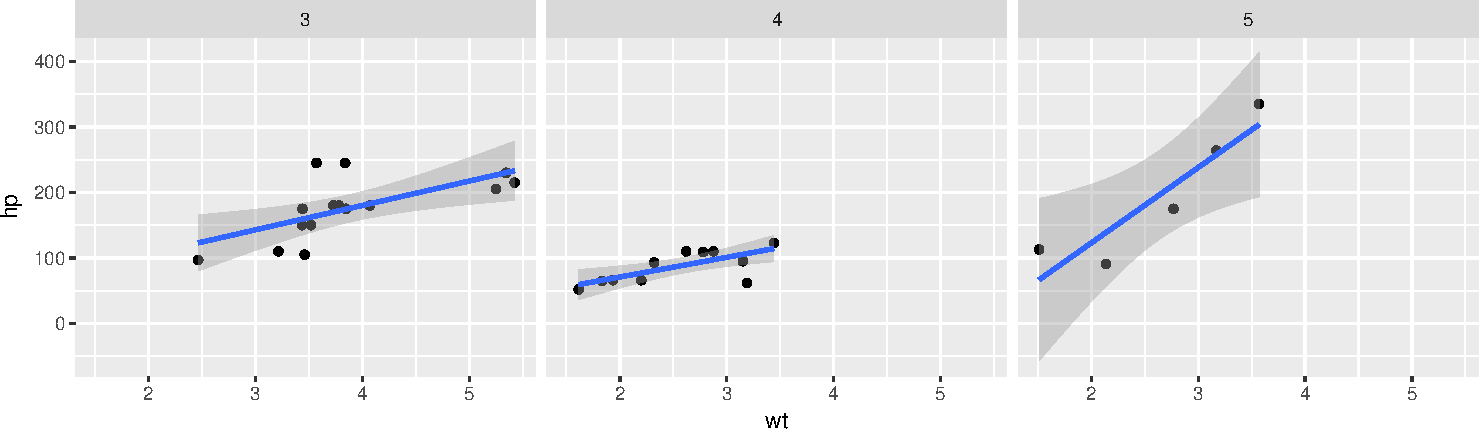
\includegraphics{../reports/APPX_A_Tech_Rpt_2017_files/figure-latex/fig-nocap-fullwidth-1} \end{figure*}

\chapter{Some Notes on Tufte CSS}\label{some-notes-on-tufte-css}

There are a few other things in Tufte CSS that we have not mentioned so
far. If you prefer \textsf<span class="sans">sans-serif fonts, use the
function \texttt{sans\_serif()} in \textbf{tufte}. For epigraphs, you
may use a pair of underscores to make the paragraph italic in a block
quote, e.g.

\begin{quote}
\emph{I can win an argument on any topic, against any opponent. People
know this, and steer clear of me at parties. Often, as a sign of their
great respect, they don't even invite me.}

\hfill<span class="blockquote footer">--- Dave Barry
\end{quote}

We hope you will enjoy the simplicity of R Markdown and this R package,
and we sincerely thank the authors of the Tufte-CSS and Tufte-LaTeX
projects for developing the beautiful CSS and LaTeX classes. Our
\textbf{tufte} package would not have been possible without their heavy
lifting.

You can turn on/off some features of the Tufte style in HTML output. The
default features enabled are:

\begin{Shaded}
\begin{Highlighting}[]
\FunctionTok{output:}
  \FunctionTok{tufte:}\AttributeTok{:tufte_html:}
    \FunctionTok{tufte_features:}\AttributeTok{ }\KeywordTok{[}\StringTok{"fonts"}\KeywordTok{,} \StringTok{"background"}\KeywordTok{,} \StringTok{"italics"}\KeywordTok{]}
\end{Highlighting}
\end{Shaded}

If you do not want the page background to be lightyellow, you can remove
\texttt{background} from \texttt{tufte\_features}. You can also
customize the style of the HTML page via a CSS file. For example, if you
do not want the subtitle to be italic, you can define

\begin{Shaded}
\begin{Highlighting}[]
\NormalTok{h3}\FloatTok{.subtitle}\NormalTok{ em }\KeywordTok{\{}
  \KeywordTok{font-style:} \DataTypeTok{normal}\KeywordTok{;}
\KeywordTok{\}}
\end{Highlighting}
\end{Shaded}

in, say, a CSS file \texttt{my\_style.css} (under the same directory of
your Rmd document), and apply it to your HTML output via the
\texttt{css} option, e.g.,

\begin{Shaded}
\begin{Highlighting}[]
\FunctionTok{output:}
  \FunctionTok{tufte:}\AttributeTok{:tufte_html:}
    \FunctionTok{tufte_features:}\AttributeTok{ }\KeywordTok{[}\StringTok{"fonts"}\KeywordTok{,} \StringTok{"background"}\KeywordTok{]}
    \FunctionTok{css:}\AttributeTok{ }\StringTok{"my_style.css"}
\end{Highlighting}
\end{Shaded}

There is also a variant of the Tufte style in HTML/CSS named
``\href{http://nogginfuel.com/envisioned-css/}{Envisoned CSS}''. This
style can be used by specifying the argument
\texttt{tufte\_variant\ =\ \textquotesingle{}envisioned\textquotesingle{}}
in \texttt{tufte\_html()}\footnote{The actual Envisioned CSS was not
  used in the \textbf{tufte} package. We only changed the fonts,
  background color, and text color based on the default Tufte style.},
e.g.

\begin{Shaded}
\begin{Highlighting}[]
\FunctionTok{output:}
  \FunctionTok{tufte:}\AttributeTok{:tufte_html:}
    \FunctionTok{tufte_variant:}\AttributeTok{ }\StringTok{"envisioned"}
\end{Highlighting}
\end{Shaded}

To see the R Markdown source of this example document, you may follow
\href{https://github.com/rstudio/tufte/raw/master/inst/rmarkdown/templates/tufte_html/skeleton/skeleton.Rmd}{this
link to Github}, use the wizard in RStudio IDE
(\texttt{File\ -\textgreater{}\ New\ File\ -\textgreater{}\ R\ Markdown\ -\textgreater{}\ From\ Template}),
or open the Rmd file in the package:

\begin{Shaded}
\begin{Highlighting}[]
\KeywordTok{file.edit}\NormalTok{(}
\NormalTok{  tufte}\OperatorTok{:::}\KeywordTok{template_resources}\NormalTok{(}
    \StringTok{'tufte_html'}\NormalTok{, }\StringTok{'..'}\NormalTok{, }\StringTok{'skeleton'}\NormalTok{, }\StringTok{'skeleton.Rmd'}
\NormalTok{  )}
\NormalTok{)}
\end{Highlighting}
\end{Shaded}

This document is also available in
\href{http://rstudio.github.io/tufte/cn/}{Chinese}, and its
\texttt{envisioned} style can be found
\href{http://rstudio.github.io/tufte/envisioned/}{here}.

\renewcommand\bibname{References}
\bibliography{skeleton.bib,/Library/Frameworks/R.framework/Versions/3.4/Resources/library/Literasee/rmarkdown/content/bibliography/Literasee.bib}



\end{document}
